\section{Definicion formal de lenguajes de modelado.
El rol del metamodelo}
Aca se habla de los mecanismos para definir la sintaxis de los lenguajes con los cuales se crean los modelos de un sistema.
\\
- Tecnicas de metamodelado.
\\
- Arquitectura de cuatro capas de modelado definida por el OMG
\\
- ¿Porque el metamodelado es tan importante en el contexte de MDD?
\\
\subsection{Mecanismos para definir la sintaxis de un lenguaje de modelado}
Hace algunos años, la sintaxis de los lenguajes se definía casi exclusivamente
usando Backus Naur Form (BNF). Este formalismo es una meta
sintaxis usada para expresar gramáticas libres de contexto, es decir,
una manera formal de describir cuáles son las palabras básicas del lenguaje
y cuáles secuencias de palabras forman una expresión correcta
dentro del lenguaje.

Usando un lenguaje de modelado,
podemos crear modelos; un modelo especifica que elementos
pueden existir en un sistema. Si se define la clase Persona en un modelo,
se pueden tener instancias de Persona como Juan, Pedro, etc. Por otro
lado, la definición de un lenguaje de modelado establece que elementos
pueden existir en un modelo. Por ejemplo, el lenguaje UML establece que
dentro de un modelo se pueden usar los conceptos Clase, Atributo, Asociación,
Paquete, etc. Debido a esta similitud, se puede describir un lenguaje
por medio de un modelo, usualmente llamado “metamodelo”. El
metamodelo de un lenguaje describe que elementos pueden ser usados
en el lenguaje y como pueden ser conectados.
Como un metamodelo es también un modelo, el metamodelo en sí mismo
debe estar escrito en un lenguaje bien definido. Este lenguaje se
llama metalenguaje. Desde este punto de vista, BNF es un metalenguaje.
En la figura 3-1 se muestra gráficamente esta relación.

\begin{figure}[H]
\centering
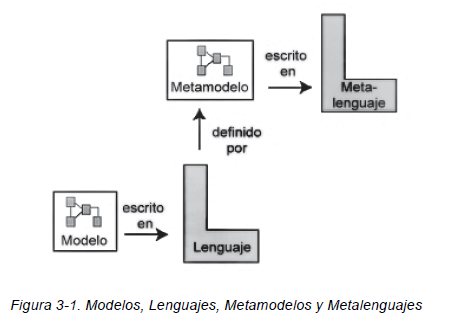
\includegraphics[scale=0.9]{./Imagenes/modelo8}
\end{figure}

\subsection{La arquitectura de 4 capas de modelado del OMG}

El metamodelado es entonces un mecanismo que permite definir formalmente
	lenguajes de modelado, como por ejemplo UML. La Arquitectura
	de cuatro capas de modelado es la propuesta del OMG orientada a
	estandarizar conceptos relacionados al modelado, desde los más abstractos
	a los más concretos.
\\
\\
\textbf{Nivel M0: Instancias}

En el nivel M0 se encuentran todas las instancias “reales” del sistema,
es decir, los objetos de la aplicación. Aquí no se habla de clases, ni
atributos, sino de entidades físicas que existen en el sistema.

\begin{figure}[H]
\centering
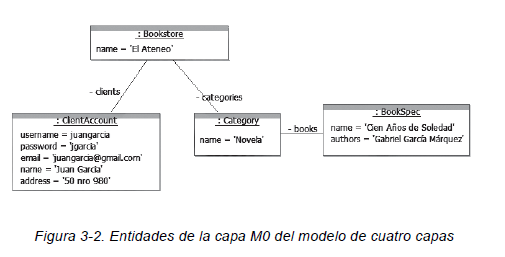
\includegraphics[scale=0.9]{./Imagenes/modelo9}
\end{figure}


\textbf{Nivel M1: Modelo del sistema}

Por encima de la capa M0 se sitúa la capa M1, que representa el modelo
de un sistema de software. Los conceptos del nivel M1 representan categorías
de las instancias de M0. Es decir, cada elemento de M0 es una
instancia de un elemento de M1. Sus elementos son modelos de los datos.

\begin{figure}[H]
\centering
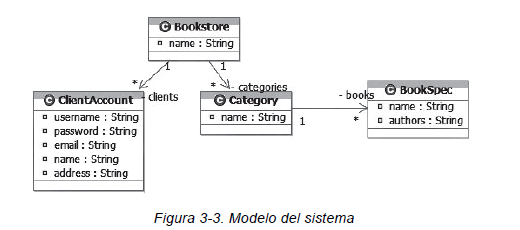
\includegraphics[scale=0.9]{./Imagenes/modelo10}
\end{figure}


\textbf{Nivel M2: Metamodelo}

Análogamente a lo que ocurre con las capas M0 y M1, los elementos del
nivel M1 son a su vez instancias del nivel M2. Esta capa recibe el nombre
de metamodelo.

\begin{figure}[H]
\centering
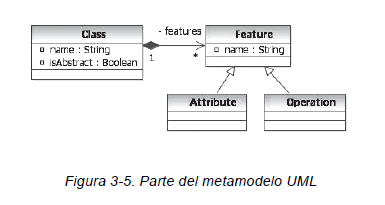
\includegraphics[scale=0.9]{./Imagenes/modelo11}
\end{figure}

Siguiendo el ejemplo, la entidad ClientAccount será una instancia de la
metaclase Class del metamodelo UML. Esta instancia tiene cinco objetos
relacionados a través de la meta asociación feature, por ejemplo una instancia
de Attribute con name=’username’ y type=’String’ y otra instancia
de Attribute con name=’password’ y type=’String’.
La figura 3-6 muestra la relación entre los elementos del nivel M1 con los
elementos del nivel M2.

\begin{figure}[H]
\centering
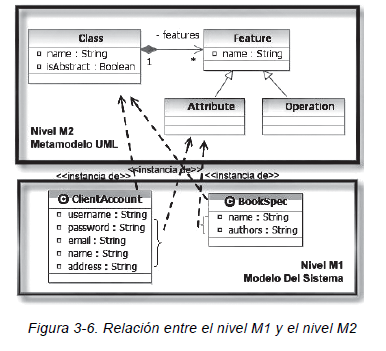
\includegraphics[scale=0.9]{./Imagenes/modelo12}
\end{figure}


\textbf{Nivel M3: Meta-metamodelo}

De la misma manera podemos ver los elementos de M2 como instancias de
otra capa, la capa M3 o capa de meta-metamodelo. Un meta-metamodelo es
un modelo que define el lenguaje para representar un metamodelo. La relación
entre un meta-metamodelo y un metamodelo es análoga a la relación
entre un metamodelo y un modelo.
M3 es el nivel más abstracto, que permite definir metamodelos concretos.
Dentro del OMG, MOF es el lenguaje estándar de la capa M3. Esto supone
que todos los metamodelos de la capa M2, son instancias de MOF.

\begin{figure}[H]
\centering
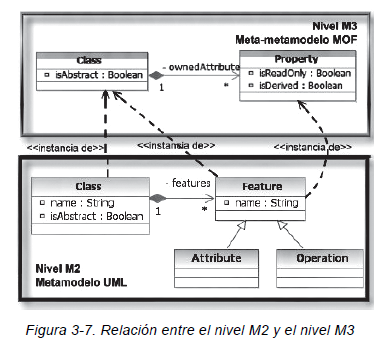
\includegraphics[scale=0.9]{./Imagenes/modelo13}
\end{figure}

\subsection{El uso del metamodelado en MDD}
Las razones por las que el metamodelado es tan importante en MDD son:

- En primer lugar, necesitamos contar con un mecanismo para definir lenguajes
de modelado sin ambigüedades [CESW 04] y permitir que una herramienta
de transformación pueda leer, escribir y entender los modelos.

- Luego, las reglas de transformación que constituyen una definición
de una transformación describen como un modelo en un lenguaje
fuente puede ser transformado a un modelo en un lenguaje destino.
Estas reglas usan los metamodelos de los lenguajes fuente y destino
para definir la transformación.

\begin{figure}[H]
\centering
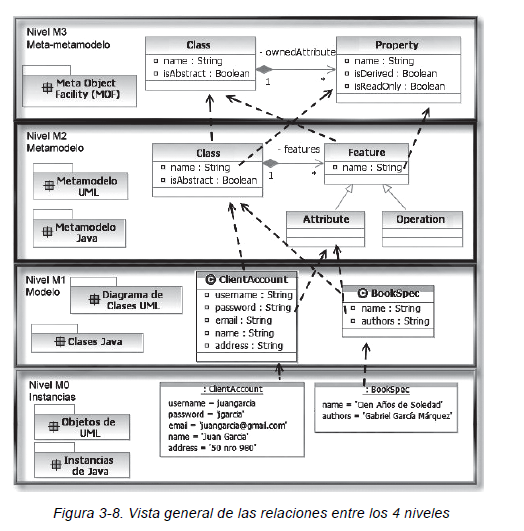
\includegraphics[scale=0.9]{./Imagenes/modelo14}
\end{figure}

- Y finalmente, la sintaxis de los lenguajes en los cuales se expresan
las reglas de transformación también debe estar formalmente definida
para permitir su automatización. En este caso también se utilizará
la técnica de metamodelado para especificar dicha sintaxis.

\begin{figure}[H]
\centering
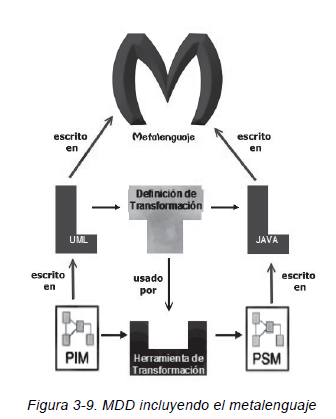
\includegraphics[scale=0.9]{./Imagenes/modelo15}
\end{figure}

\subsection{El lenguaje de modelado más abstracto: MOF}

El lenguaje MOF, acrónimo de Meta-Object Facility, es un estándar del
OMG para la ingeniería conducida por modelos. Como se vio anteriormente,
MOF se encuentra en la capa superior de la arquitectura de 4
capas. Provee un meta-meta lenguaje que permite definir metamodelos
en la capa M2. El ejemplo más popular de un elemento en la capa M2 es
el metamodelo UML, que describe al lenguaje UML.
Esta es una arquitectura de metamodelado cerrada y estricta.

\begin{figure}[H]
\centering
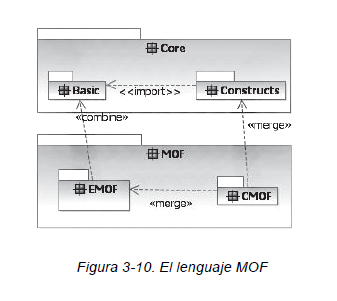
\includegraphics[scale=0.9]{./Imagenes/modelo16}
\end{figure}


\subsection{Ejemplos de metamodelos}

MOF puede ser usado para definir metamodelos de lenguajes orientados
a objetos, como es el caso de UML, y también para otros lenguajes
no orientados a objetos, como es el caso de las redes de Petri o los
lenguajes para servicios web.
En esta sección mostramos algunos ejemplos de metamodelos, en
particular la figura 3-12 muestra el metamodelo simplificado del lenguaje
UML donde se especifica que un modelo UML está formado por
paquetes (Package), donde cada paquete está integrado por clases
(Clase) que poseen atributos (Attribute). Los atributos tienen un nombre
(name) y un tipo (type), que puede ser un tipo de dato primitivo
(PrimitiveDataType) o una clase.

\begin{figure}[H]
\centering
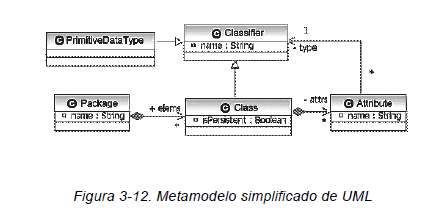
\includegraphics[scale=0.9]{./Imagenes/modelo17}
\end{figure}

El metamodelo del lenguaje RDBMS que mostramos en la figura 3-13
indica que un modelo relacional consta de esquemas (Schema), donde
cada esquema está compuesto por tablas (Table) que tienen columnas
(Column). Las columnas tienen un nombre (name) y un tipo de dato
(type). La tabla tiene una clave primaria (pkey) y cero o más claves
foráneas (fkeys). Cada clave foránea (Kkey) hace referencia a columnas
en otras tablas.

\begin{figure}[H]
\centering
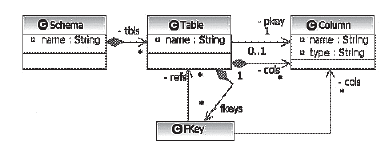
\includegraphics[scale=0.9]{./Imagenes/modelo18}
\end{figure}

